\documentclass[main.tex]{subfiles}

\usepackage[clean]{svg}
\usepackage{svg}
\usepackage{amsmath}

\usepackage{pdfpages}

\begin{document}

\section{Regresija}
\label{sec:regresija}

Regresija predstavlja tehniku za modelovanje veze između zavisne (ciljne) promenljive i jedne ili više nezavisnih promenljivih (atributa). Pripada grupi algoritama mašinskog učenja koji se zasnivaju na nadgledanom učenju. 

Kod algoritama nadgledanog učenja za svaki uzorak iz skupa za trening data je i tačna izlazna vrednost za taj uzorak. Podaci o izlaznim vrednostima koriste se u obuci algoritama koji će za neki novi neobeleženi uzorak predvideti vrednost izlaza. Problemi nadgledanog učenja se nazivaju regresionim ukoliko je izlazna promenljiva kontinualnog tipa. U ovom slučaju cilj je formiranje modela koji će na osnovu dostupnih uzoraka za trening i odgovarajućih izlaznih vrednosti predvidati vrednost kontinualne izlazne promenljive za novi uzorak.

Pošto se regesija uglavnom koristi za predviđanje vrednosti, modelovanje vremenskih serija i određivanje uzročno-posledičnih veza između promenljivih, ima primenu u različitim oblastima, poput finansija, marketinga, fizike i biologije.

Postoje različiti tipovi regresione analize, poput linearne regresije, polinomijalne regresije i simboličke regresije.


\subsection{Linearna regresija}
\label{sec:linearnaRegresija}

Jedan od najjednostavnijih i najčešće korišćenih tipova regresije je linearna regresija. Linearna regresija predstavlja metodu nadgledanog učenja koja se koristi za predviđanje vrednosti kontinualne izlazne promenljive uz pretpostavku da se ta vrednost može dobiti kao linearna kombinacija vrednosti ulaznih obeležja. Formiranje modela linearne regresije svodi se na određivanje parametara pretpostavljene linearne zavisnosti.

Kako model linearne regresije pretpostavlja linearnu zavisnost po parametrima $\beta_0$, $\beta_1$, ..., $\beta_m$ između atributa $x_1$, $x_2$, ..., $x_m$ i ciljne promenljive $y$, onda se $y$ predstavlja u obliku

\[ y = \beta_0 + \beta_1 x_1 + \beta_2 x_2 + ... + \beta_m x_m .\]

Geometrijski posmatrano, cilj linearne regresije je pronalazak prave koja najbolje opisuje date podatke. Na slici \ref{fig:linReg} se može videti primer proste linarne regresije predstavljene modelom $f(x) = \beta_0 + \beta_1 x$.


\begin{figure}[!ht]
\begin{center}
\includegraphics[width=0.5\textwidth]{../images_pdf/linear_regression.pdf}
\end{center}
\caption{Linearna regresija}
\label{fig:linReg}
\end{figure}


%\begin{figure}[!ht]
%\begin{center}
%\includepdf[pages={1},scale=0.4]{../images_svg/linear_regression.pdf}
%\end{center}
%\caption{Linearna regresija}
%\label{fig:linReg}
%\end{figure}



\subsection{Polinomijalna regresija}
\label{sec:polinomijalnaRegresija}

Polinomijalna regresija je tip regresione analize kod koje se veza između atributa i ciljne promenljive modeluje pomoću polinoma $n$-tog stepena. U slučaju jedne nezavisne promenljive, ciljna promenljiva je oblika

\[ y = \beta_0 + \beta_1 x_1 + \beta_2 x_1^{2} + ... + \beta_m x_1^{m} \] \\

Na slici \ref{fig:polyReg} može se videti uporedni prikaz proste linearne i polinomijalne regresije.

\begin{figure}[!ht]
\begin{center}
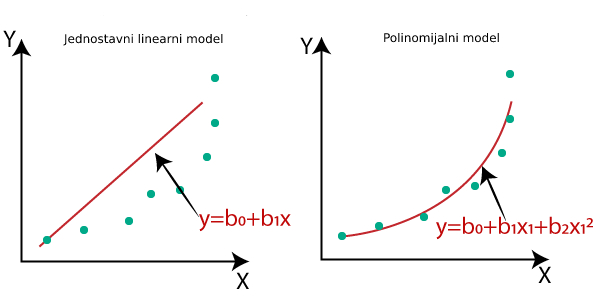
\includegraphics[width=0.55\textwidth]{../images/polynomial_regression.jpg}
\end{center}
\caption{Polinomijalna regresija}
\label{fig:polyReg}
\end{figure}

Ovakav model se i dalje smatra linearnim, jer su težine pridružene atributima linearne. Samo je kriva koju modelujemo polinomijalnog obilka.

\subsection{Simbolička regresija}
\label{sec:SR}

Simbolička regresija predstavlja generalizaciju linearne ili polinomijalne regresije. Dok one pretpostavljaju linearnu ili polinomijalnu formu modela i optimizuju samo numeričke parametre tog predefinisanog modela, simbolička regresija istovremeno uči i o strukturi modela i njegove parametre. Upravo zbog toga što ne zahteva prethodnu specifikaciju strukture modela, na simboličku regresiju manje utiču ljudske greške i nedovoljno domensko znanje.

U suštini, cilj simboličke regresije je pronalazak matematičkog izraza u simboličkoj formi, koji dobro modeluje vezu između ciljne promenljive i nezavisnih promenljivih. 

%Formalno, ako je dat skup podataka $(X, y)$, gde $X_i \in \mathcal{R}^{n}$ predstavlja skup atributa, a $y_i \in \mathcal{R}$ ciljnu promenljivu, cilj simboličke regresije je pronalazak funkcije $f: \mathcal{R}^{n} \rightarrow \mathcal{R}$ koja najbolje odgovara skupu podataka.

Formalno, ako je dat skup podataka $(X_i, y_i)$, $i=1,...,n$, gde $X_i \in \mathbb{R}^{n}$ predstavlja $i$-ti skup atributa, a $y_i \in \mathbb{R}$ $i$-tu ciljnu promenljivu, cilj simboličke regresije je pronalazak funkcije $f: \mathbb{R}^{n} \rightarrow \mathbb{R}$ koja najbolje odgovara skupu podataka, odnosno za koju važi $y_i \approx f(X_i), i=1,...,n$.

Za formiranje modela, koji pronalazi tu vezu, mogu se koristiti i različite metode dubokog učenja. Međutim, modeli formirani tim tehnikama su u vidu crne kutije i teški su za interpretaciju. Prednost simboličke regresije je u tome što je naučeni model lakše interpretirati, što može biti značajno u nekim oblastima primene koje zahtevaju mogućnost objašnjenja odluke koja je doneta pomoću tog modela. Na primer, ako se u bankarstvu odluka o izdavanju kredita donosi na osnovu modela, može biti potrebno obrazloženje donete odluke, pogotovo ako je korisnik odbijen. 

Takođe, model dobijen simboličkom regresijom se može dalje analizirati. Pošto se radi o matematičkoj funkciji, moguće je, na primer, odrediti njenu periodičnost, asimptotsko ponašanje ili bilo koju drugu osobinu koja može biti od značaja za posmatranu oblast.


\section{Evaluacija regresionih modela}
\label{sec:evaluacija}

Za evaluaciju regresionih modela, pa tako i modela simboličke regresije, mogu se koristiti različite metrike, poput srednje kvadratne greške i koeficijenta određenosti $R^{2}$, takođe poznatog i pod nazivom koeficijent determinacije (eng. \textit{coefficient of determination}).  
Srednje kvadratna greška se izražava u terminima veličine ciljne promenljive, dok
je vrednost koeficijenta određenosti normirana.

Srednje kvadratna greška (MSE, eng. \textit{Mean Squared Error}) se izražava kao

 \[ MSE = \frac{1}{n} \sum_{i=1}^{n}(y_i - \hat{y_i})^{2}, \]
 gde je $n$ broj uzoraka, $y_i$ stvarna vrednost ciljne promenljive za $i$-ti uzorak, a $\hat{y_i}$ predviđena vrednost.
 
 Vrednost MSE je uvek pozitivna, pri čemu vrednost bliža nuli označava kvalitetniji model.
 
 Vizualna reprezentacija srednje kvadratne greške je prikazana na slici \ref{fig:MSE}.

\begin{figure}[!ht]
\begin{center}
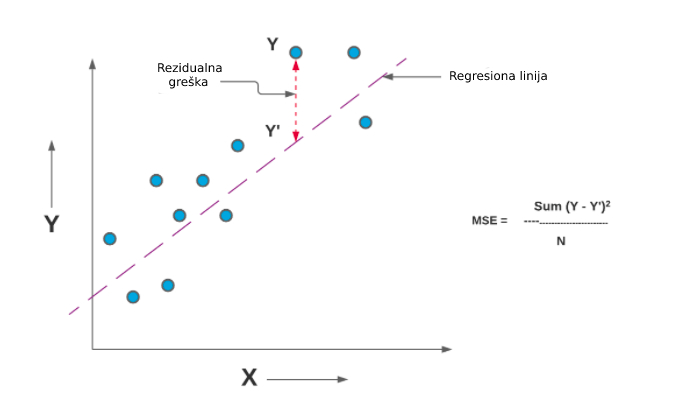
\includegraphics[width=0.7\textwidth]{../images/mse.jpg}
\end{center}
\caption{Vizualna reprezentacija srednje kvadratne greške}
\label{fig:MSE}
\end{figure}

 
 \iffalse
 Koeficijent određenosti izračunava udeo varijanse ciljne promenljive koji je objašnjen naučenim modelom, tj. pokazuje kako variraju vrednosti ciljne promenljive kada variraju vrednosti atributa. Izračunava se kao
 
 \[ R^{2} = 1 - \frac{\sum_{i=1}^{n}(y_i - \hat{y_i})^{2}}{\sum_{i=1}^{n}(y_i - \bar{y})^{2}}, \]
 gde je $\bar{y}$ prosek ciljne promenljive uzorka.
\fi
 
Koeficijent određenosti se izračunava kao količnik zbira kvadrata regresije (SSR, eng. \textit{Sum of Squares Regression}) i ukupnog zbira kvadrata (SST, eng. \textit{Sum of Squares Total}). SSR predstavlja varijansu predviđenih vrednosti koje se nalaze na regresionoj pravoj ili ravni u odnosu na srednju vrednost ciljne promenljive iz uzorka. SST predstavlja varijansu stvarnih vrednosti ciljne promenljive u odnosu na srednju vrednost ciljne promenljive iz uzorka. Odnosno, koeficijent određenosti se izračunava kao

\[ R^{2} = \frac{SSR}{SST} = \frac{\sum_{i=1}^{n}(\hat{y_i} - \bar{y})^{2}}{\sum_{i=1}^{n}(y_i - \bar{y})^{2}}, \]
gde je $\bar{y}$ srednja vrednost ciljne promenljive iz uzorka, $\hat{y_i}$ predviđena vrednost ciljne promenljive, a $y_i$ stvarna vrednost ciljne promenljive.

Što je veća $R^{2}$ vrednost, to je i naučeni model bolji, jer je njime objašenjen veći udeo varijanse ciljne promenljive u odnosu na srednju vrednost.

$R^{2}$ se može izraziti i preko SSE greške (eng. \textit{Sum of Squares Error}). SSE predstavlja deo varijanse koja nije obuhvaćena modelom. U tom slučaju važi

%\[ R^{2} = 1 - \frac{SSE}{SST} = 1 - \frac{\sum_{i=1}^{n}(y_i - \hat{y_i})^{2}}{\sum_{i=1}^{n}(y_i - \bar{y})^{2}}. \]

\[
\begin{aligned}
R^{2} &=1-\frac{S S E}{S S T} \\
&=1-\frac{\sum_{1=1}^{n}\left(y_i-\hat{y_i}\right)^{2}}{\left. \sum_{i=1}^{n}(y_i-\bar{y}\right)^{2}} \\
&=1-\frac{\frac{1}{n} \sum_{1=1}^{n}\left(y_i-\hat{y_i}\right)^{2}}{\left.\frac{1}{n} \sum_{i=1}^{n}(y_i-\bar{y}\right)^{2}} \\
&=1-\frac{MSE}{\operatorname{Var}(y)}
\end{aligned}.
\]

Lako se uočava da veća vrednost $R^{2}$ znači manju MSE vrednost.

Dok na skupu podataka za trening $R^{2}$ uzima vrednosti iz intervala [0, 1], na skupu podataka za test može da se desi da vrednost bude i negativna (u slučaju kada je SSE veće od SST), što ukazuje da se radi o vrlo lošem modelu.

Vizualna reprezentacija koeficijenta određenosti je prikazana na slici \ref{fig:R2}.

\begin{figure}[!ht]
\begin{center}
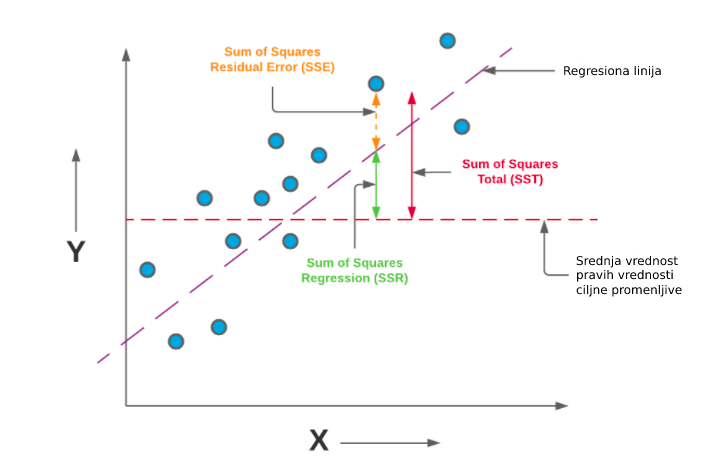
\includegraphics[width=0.8\textwidth]{../images/rSquared.jpg}
\end{center}
\caption{Vizualna reprezentacija koeficijenta određenosti}
\label{fig:R2}
\end{figure}


\section{Reprezentacija izraza kod simboličke regresije}
\label{sec:expressionRepr}

Postoje različiti načini na koje mogu da se predstave matematički izrazi sa kojima se operiše u okviru simboličke regresije. Na primer, izraz se može konstruisati pomoću pravila kontekstno-slobodnih gramatika \cite{grammarForEquationDiscovery, abstractExprGrammar, automaticGrammaticalEvolution} ili se može predstaviti u vidu sintaksnog stabla \cite{koza, semanticCrossover, beeColony, vnp}. Pošto će u ovom radu biti korišćena reprezentacija pomoću sintaksnog stabla, u nastavku će biti prikazan samo taj pristup.

Pomoću sintaksnog stabla izraz se obično predstavlja u prefiksnoj notaciji. Listovi sintaksnog stabla mogu da sadrže samo terminale izraza, odnosno mogu predstavljati konstante i nezavisne promenljive iz datog skupa podataka. Unutrašnjim čvorovima stabla su predstavljene unarne i binarne funkcije (npr. +, -, sin, cos, log, ...).
U okviru jednog stabla ista funkcija se može pojaviti veći broj puta. Isto važi i za konstante i promenljive.
Dodatno, skupovi funcija i terminala su fiksirani u skladu sa trenutnim problemom koji se rešava.

Slika \ref{fig:syntaxTree1} ilustruje primer sintaksnog stabla za izraz

\[ \max \left\{\frac{3}{x_{3} * 2.4} ; x_{1}-x_{2}\right\} \]


\begin{figure}[!ht]
\begin{center}
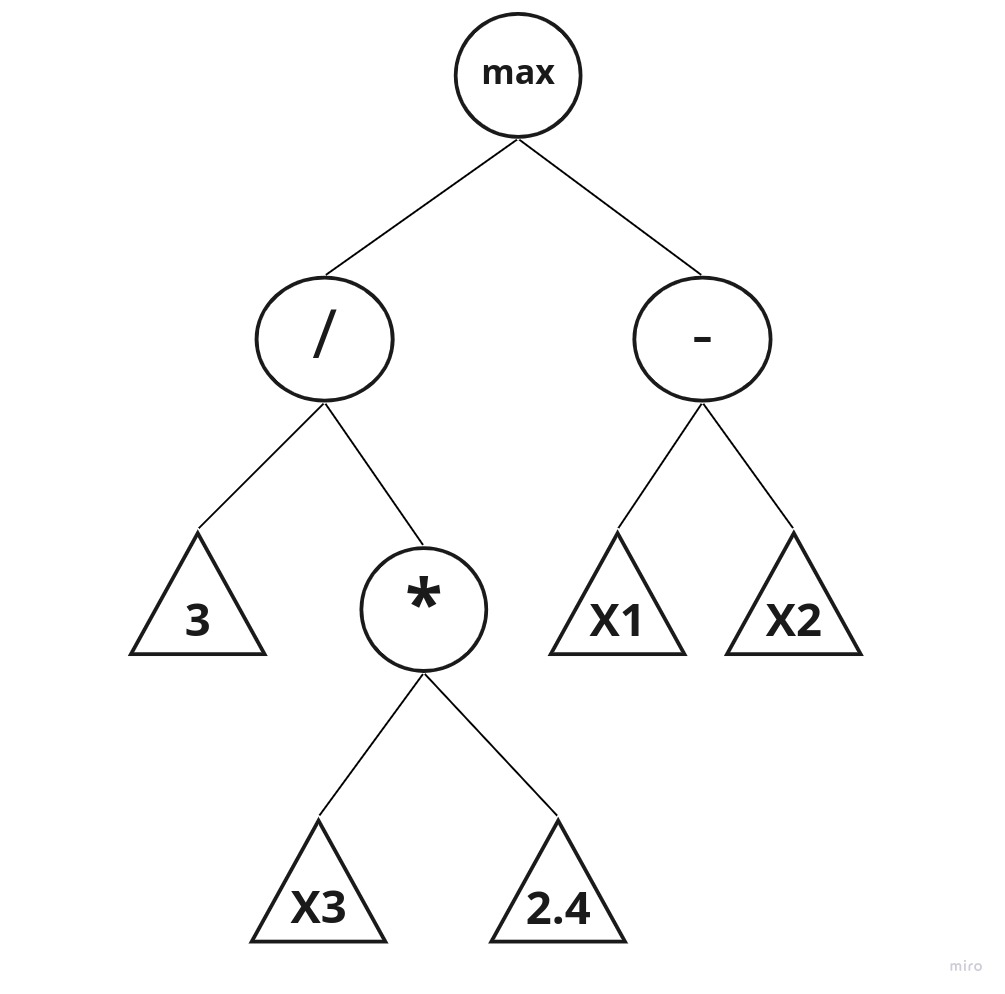
\includegraphics[width=0.4\textwidth]{../images/syntax_tree.jpg}
\end{center}
\caption{Primer sintaksnog stabla}
\label{fig:syntaxTree1}
\end{figure}

Prilikom ocenjivanja tačnosti regresionog modela treba uzeti u obzir da se jedna ista funkcija može izraziti pomoću više simbolički različitih zapisa. Na primer, ako je ciljna funkcija $f$ jednaka $(u + v) / (1 + uv/c^{2})$ onda se i simbolički različit zapis $(v + u) / (1 + uv/c^{2})$ treba smatrati tačnim rešenjem. Odnosno, smatra se da je ciljna funkcija $f$ ispravno određena kandidatskom funkcijom $f'$ ako algebarska simplifikacija izraza $f' - f$ daje simbol "0" \cite{AIFeynman}. 


\section{Simbolička regresija kao NP-težak problem}
\label{sec:np}

Razlikujemo sledeće klase složenosti:
\begin{itemize}
\item \textbf{Klasa P.} Ovoj klasi pripadaju svi problemi za koje postoji algoritam polinomske složenosti koji ga rešava.
\item \textbf{Klasa NP.} Ovoj klasi pripadaju svi problemi za koje se može izvršiti provera rešenja u polinomskom vremenu. Jasno je da je $P \subset NP$, međutim za sada nije poznato da li je i $NP \subset P$. Problem određivanja da li je $P \neq NP$ je jedan od najpoznatijih otvorenih problema u teorijskom računarstvu.
\item \textbf{NP-teški problemi.} Problem je NP-težak ako se svaki problem iz klase NP može u polinomskom vremenu redukovati na njega. Da bi se dokazalo da je problem NP-težak, dovoljno je dokazati da postoji polinomska redukcija bar jednog NP-teškog problema na njega.
\item \textbf{NP-kompletni problemi.} Problem je NP-kompletan ukoliko pripada klasi NP i ukoliko je NP-težak.
\end{itemize}

Problem simboličke regresije se smatra problemom kombinatorne optimizacije.

Kako je prostor matematičkih izraza diskretan (u smislu strukture modela) i kontinualan (u smislu parametara modela, npr. konstante mogu biti realni brojevi), prostor pretrage se može eksponencijalno povećati sa povećanjem dužine izraza.

Zbog navedenih karakteristika, postavljena je hipoteza da je simbolička regresija NP-težak problem, međutim to još uvek nije formalno dokazano \cite{np-hard1, np-hard2}. Ali, pošto je instance velikih dimenzija praktično nemoguće rešiti usled ograničenja vremenskih i memorijskih resursa, najčešće se traže aproksimativna rešenja poroblema, uglavnom pomoću razlčitih metaheurističkih metoda.

\end{document}